\documentclass[[12pt,twoside]{book}
\usepackage{_my_document_style}
\begin{document}
\begin{figure}[t]%[H]%[!htbp]
  \centering
  %\checkoddpage
  %\centering
    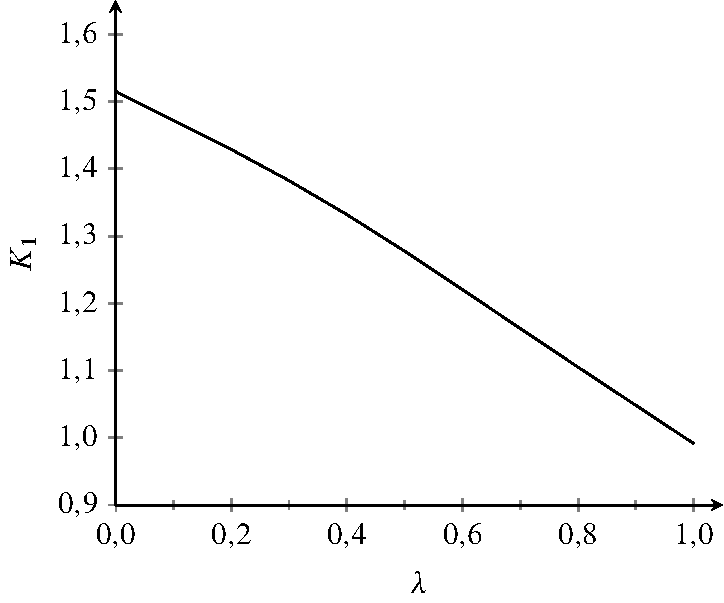
\includegraphics[width=0.65\textwidth]{Chapter_2/aerodynamic_center_of_a_finite_wing/plot_wing_ac_K1_vs_lambda.pdf}%
  \caption{\finalhyphendemerits=1000
           Coefficient $K_1$ in the aerodynamic center calculation formula of a finite wing.}
  \label{fig:Wing:Ac:K:One:Plots}%
\end{figure}

\begin{myExampleX}{Aerodynamic center of a wing with straight edges, tapered and swept}{\ding{46}\ \myIconGraph\ }% \ \Keyboard\ %
\label{example:Wing:Aerodynamic:Center:Of:A:Finite:Wing}
%
\def\mySpanWingMT{26.800000}
\def\myChordRootWingMT{5.200000}
\def\myChordTipWingMT{1.600000}
\def\myTaperRatioWing{0.307692}
\def\myAreaWingMTsquared{91.120000}
\def\myMACWingMT{3.717647}
\def\myYMACWingMT{5.517647}
\def\myXMACLEToApexWingMT{2.872305}
\def\mySweepLEWingDEG{27.500000}
\def\mySweepLEWingRAD{0.479966}
\def\myAspectRatioWing{7.882353}
\def\myMach{0.700000}
\def\myKOneACDatcomWing{1.395000}
\def\myKTwoACDatcomWing{-0.268657}
\def\myXACOverChordRootDatcomWing{0.758000}
\def\myXsiACWing{0.279000}
\def\myXACOverChordRootDatcomWing{3.909529}

%
\noindent
Consider the wing assigned in the example~\ref{example:Geometric:Characteristics:Of:A:Wing:With:Sweep:Angle:Not:Null}.
With the help of the graphs shown in the figures~\ref{fig:Wing:Ac:K:One:Plots},
\ref{fig:Wing:Ac:K:Two:Plots} and~\ref{fig:Wing:Ac:X:AC:From:Apex:Plots}, we want to calculate
the position of the aerodynamic center for a flight Mach number
$\Mach = \SI[round-precision=2]{\myMach}{}$.

\medskip
From the data and the figure~\ref{fig:Wing:Ac:K:One:Plots}
we obtain
\[
\lambda=\SI[round-precision=2]{\myTaperRatioWing}{}
%
%\quad \Longrightarrow \quad
%\quad \begin{array}{@{}c@{}} \myIconGraph \\[-4pt] \Longrightarrow \end{array} \quad
\adjustbox{center=4em}{%
  \adjustbox{lap=\width}{\raisebox{2.2ex}[0pt][0pt]{\myIconGraph}}$\Longrightarrow$%
}
%
K_1
  = \mathunderline{mydarkblue}{ \SI[round-precision=3]{\myKOneACDatcomWing}{} }
\]
from the figure~\ref{fig:Wing:Ac:K:Two:Plots}
we get
\[
\Lambda_\mathrm{le} = \SI[round-precision=1]{\mySweepLEWingDEG}{\deg}\;,\;\,
\AR = \SI[round-precision=1]{\myAspectRatioWing}{}\;,\;\,
\lambda=\SI[round-precision=2]{\myTaperRatioWing}{}
%\quad \Longrightarrow \quad
%\quad \begin{array}{@{}c@{}} \myIconGraph \\[-4pt] \Longrightarrow \end{array} \quad
\adjustbox{center=4em}{%
  \adjustbox{lap=\width}{\raisebox{2.2ex}[0pt][0pt]{\myIconGraph}}$\Longrightarrow$%
}
%
K_2 
  = \mathunderline{mydarkblue}{ \SI[round-precision=3]{\myKTwoACDatcomWing}{} }
\]
from the figure~\ref{fig:Wing:Ac:X:AC:From:Apex:Plots}
we get
\[
\Lambda_\mathrm{le} = \SI[round-precision=1]{\mySweepLEWingDEG}{\deg}\;,\;\,
\Mach = \SI[round-precision=2]{\myMach}{}\;,\;\,
\AR = \SI[round-precision=1]{\myAspectRatioWing}{}\;,\;\,
\lambda=\SI[round-precision=2]{\myTaperRatioWing}{}
%
%\quad \Longrightarrow \quad
%\quad \begin{array}{@{}c@{}} \myIconGraph \\[-4pt] \Longrightarrow \end{array} \quad
\adjustbox{center=4em}{%
  \adjustbox{lap=\width}{\raisebox{2.2ex}[0pt][0pt]{\myIconGraph}}$\Longrightarrow$%
}
%
\frac{X'_{\mathrm{ac}}}{c_\mathrm{r}}
  = \mathunderline{mydarkblue}{ \SI[round-precision=3]{\myXACOverChordRootDatcomWing}{} }
\]
%
It is thus obtained
\[
\frac{x_{\mathrm{ac}}}{\bar{c}} 
  = K_1 \left( \frac{X'_{\mathrm{ac}}}{c_\mathrm{r}} - K_2  \right)
  = \SI[round-precision=3]{\myKOneACDatcomWing}{} \,
    \Big(  
      \SI[round-precision=3]{\myXACOverChordRootDatcomWing}{} 
        - \SI[round-precision=3]{\myKTwoACDatcomWing}{}  
    \Big)
  = \mathunderline{mydarkblue}{ \SI[round-precision=3]{\myXsiACWing}{} } 
\]

The graphic representation of the aerodynamic center of the assigned wing
$(X_\mathrm{ac},0)$ is given by the figure~\ref{fig:Wing:Aerodynamic:Center:Results:A}.
The position of $X_\mathrm{ac}$ is easily calculated as
\[
\begin{split}
X_\mathrm{ac} & {}= X_{\mathrm{le},\bar{c}} + \left( \frac{x_{\mathrm{ac}}}{\bar{c}} \right) \bar{c}
\\
  & {}=
    \SI[round-precision=2]{\myXMACLEToApexWingMT}{\metre}
      + \SI[round-precision=3]{\myXsiACWing}{}
        \cdot \SI[round-precision=2]{\myMACWingMT}{\metre}
      = \SI[round-precision=2]{\myXMACLEToApexWingMT}{\metre}
        + \calcSI[round-precision=2]{\myXsiACWing*\myMACWingMT}{\metre}
    = \mathunderline{mydarkblue}{ 
      \calcSI[round-precision=2]{\myXMACLEToApexWingMT + \myXsiACWing*\myMACWingMT}{\metre} 
    }%
\end{split}
\]
\end{myExampleX}
%-----------------------------------------------------------------------------------------------
\begin{figure}[t]%[H]%[!htbp]
  %\centering
  %\checkoddpage
  %\centering
    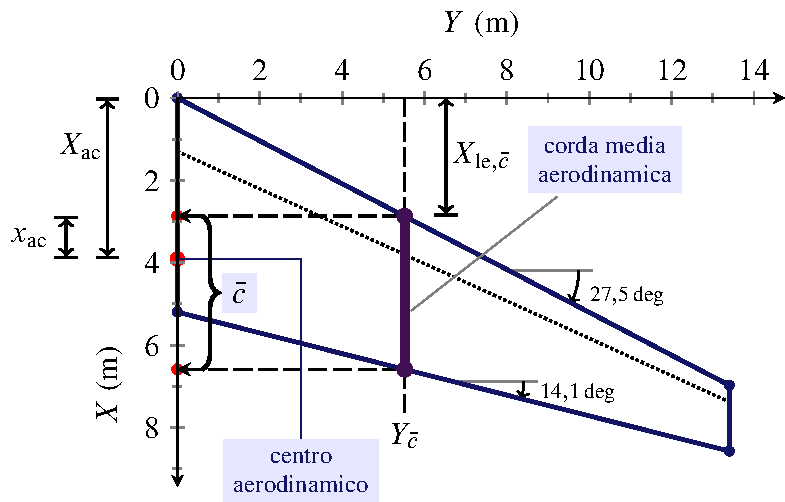
\includegraphics[width=0.70\textwidth]{Chapter_2/aerodynamic_center_of_a_finite_wing/wing_ac_1_drawing.pdf}%
  \caption{\finalhyphendemerits=1000
        Aerodynamic center of the wing assigned in the example~\ref{example:Wing:Aerodynamic:Center:Of:A:Finite:Wing}.}
  \label{fig:Wing:Aerodynamic:Center:Results:A}%
\end{figure}%
%-----------------------------------------------------------------------------------------------
\EnlargedFigureX% needs two latex passes
  {p}% #1: t, b, p
  {%
    \centering
    \begin{tabular}{@{}c@{\rule{3mm}{0pt}}c@{}}
      \includegraphics%
        %[width=0.52\textwidth]
        %[height=5.5cm]
        [width=0.485\textwidth]%
        {Chapter_2/aerodynamic_center_of_a_finite_wing/plot_wing_ac_K2_lam0.pdf}
      &
      \includegraphics%
        %[width=0.52\textwidth]
         %[height=5.5cm]
        [width=0.485\textwidth]%
        {Chapter_2/aerodynamic_center_of_a_finite_wing/plot_wing_ac_K2_lam02.pdf}
      \\
      \includegraphics%
        %[width=0.52\textwidth]
        %[height=5.5cm]
        [width=0.485\textwidth]%
        {Chapter_2/aerodynamic_center_of_a_finite_wing/plot_wing_ac_K2_lam04.pdf}
      &
      \includegraphics%
      %[width=0.52\textwidth]
     %[height=5.5cm]
       [width=0.485\textwidth]%
        {Chapter_2/aerodynamic_center_of_a_finite_wing/plot_wing_ac_K2_lam06.pdf}
      \\
      \includegraphics%
        %[width=0.52\textwidth]%
         % [height=5.5cm]
     [width=0.485\textwidth]
      {Chapter_2/aerodynamic_center_of_a_finite_wing/plot_wing_ac_K2_lam08.pdf}
      &
      \includegraphics%
        %[width=0.52\textwidth]
        % [height=5.5cm]
        [width=0.485\textwidth]%
        {Chapter_2/aerodynamic_center_of_a_finite_wing/plot_wing_ac_K2_lam1.pdf}
    \end{tabular}
  }% #2: the image file included by \includegraphics
  {\finalhyphendemerits=1000
    Coefficient $K_2$ in the aerodynamic center calculation formula of a finite wing.%
  }% #3: the caption text
  {fig:Wing:Ac:K:Two:Plots}%% #4: the label
%-----------------------------------------------------------------------------------------------
\EnlargedFigureX% 
  {p}% #1: t, b, p
  {%
    \centering
    \begin{tabular}{@{}c@{\rule{3mm}{0pt}}c@{}}
      \includegraphics%
        %[width=0.52\textwidth]%
        % [height=5.5cm]%
        [width=0.485\textwidth]%
        {Chapter_2/aerodynamic_center_of_a_finite_wing/plot_xbar_prime_wing_ac_lam0.pdf}
      &
      \includegraphics%
        %[width=0.52\textwidth]%
        % [height=5.5cm]%
        [width=0.485\textwidth]%
        {Chapter_2/aerodynamic_center_of_a_finite_wing/plot_xbar_prime_wing_ac_lam02.pdf}
      \\
      \includegraphics%
        %[width=0.52\textwidth]%
        % [height=5.5cm]%
        [width=0.485\textwidth]%
        {Chapter_2/aerodynamic_center_of_a_finite_wing/plot_xbar_prime_wing_ac_lam025.pdf}
      &
      \includegraphics%
        %[width=0.52\textwidth]%
        % [height=5.5cm]%
        [width=0.485\textwidth]%
        {Chapter_2/aerodynamic_center_of_a_finite_wing/plot_xbar_prime_wing_ac_lam033.pdf}
      \\
      \includegraphics%
        %[width=0.52\textwidth]%
        % [height=5.5cm]%
        [width=0.485\textwidth]%
        {Chapter_2/aerodynamic_center_of_a_finite_wing/plot_xbar_prime_wing_ac_lam05.pdf}
      &
      \includegraphics%
        %[width=0.52\textwidth]%
        % [height=5.5cm]%
        [width=0.485\textwidth]%
        {Chapter_2/aerodynamic_center_of_a_finite_wing/plot_xbar_prime_wing_ac_lam1.pdf}
    \end{tabular}
  }% #2: the image file included by \includegraphics
  {\finalhyphendemerits=1000
    Dimensionless position $X'_\text{ac}/c_\text{r}$ in the aerodynamic center calculation formula
    of a finite wing.%
  }% #3: the caption text
  {fig:Wing:Ac:X:AC:From:Apex:Plots}%% #4: the label
\end{document}